\documentclass[twocolumn,superscriptaddress,showpacs,preprintnumbers,amsmath,amssymb,prl]{revtex4}
\usepackage{graphicx}
\usepackage{dcolumn,xcolor,ulem}
\usepackage{amsmath} 
\usepackage{amssymb}
\usepackage{amsfonts}
\usepackage{bm}
\usepackage[latin1]{inputenc}
%\usepackage{mathrsfs}

\newcommand{\cor}[1]{\textcolor{red}{#1}}
\newcommand{\change}[1]{\textcolor{blue}{#1}}
\newcommand\gp{\dot\gamma}
\newcommand\gl{\gamma_{\rm loc}}
\newcommand\gpm{\dot\gamma_{\rm min}}
\newcommand\taum{\tau_{\rm min}}

\begin{document}

%\widowpenalty=1000
%\clubpenalty=1000
%\preprint{APS/123-QED}

\title{Creep and failure of a model soft solid}

\author{M.~Leocmach}
\email{mathieu.leocmach@ens-lyon.fr}
\affiliation{Universit\'e de Lyon, Laboratoire de Physique, \'Ecole Normale Sup\'erieure de Lyon, CNRS UMR 5672, 46 All\'ee d'Italie, 69364 Lyon cedex 07, France}
\author{C.~Perge}
\affiliation{Universit\'e de Lyon, Laboratoire de Physique, \'Ecole Normale Sup\'erieure de Lyon, CNRS UMR 5672, 46 All\'ee d'Italie, 69364 Lyon cedex 07, France}
\author{N.~Taberlet}
\affiliation{Universit\'e de Lyon, Laboratoire de Physique, \'Ecole Normale Sup\'erieure de Lyon, CNRS UMR 5672, 46 All\'ee d'Italie, 69364 Lyon cedex 07, France}
\affiliation{UFR de Physique, Universit\'e Claude Bernard Lyon 1, 43 boulevard du 11 novembre, 69100 Villeurbanne, France}
\author{T.~Divoux}
\affiliation{Centre de Recherche Paul Pascal, CNRS UPR 8642 - 115 avenue Schweitzer, 33600 Pessac, France}
\author{S.~Manneville}
\affiliation{Universit\'e de Lyon, Laboratoire de Physique, \'Ecole Normale Sup\'erieure de Lyon, CNRS UMR 5672, 46 All\'ee d'Italie, 69364 Lyon cedex 07, France}

\date{\today}

\begin{abstract}
Yoghurts.
\end{abstract}

\pacs{}
\maketitle


%%%%%%%%%%%%
\begin{figure}
\centering
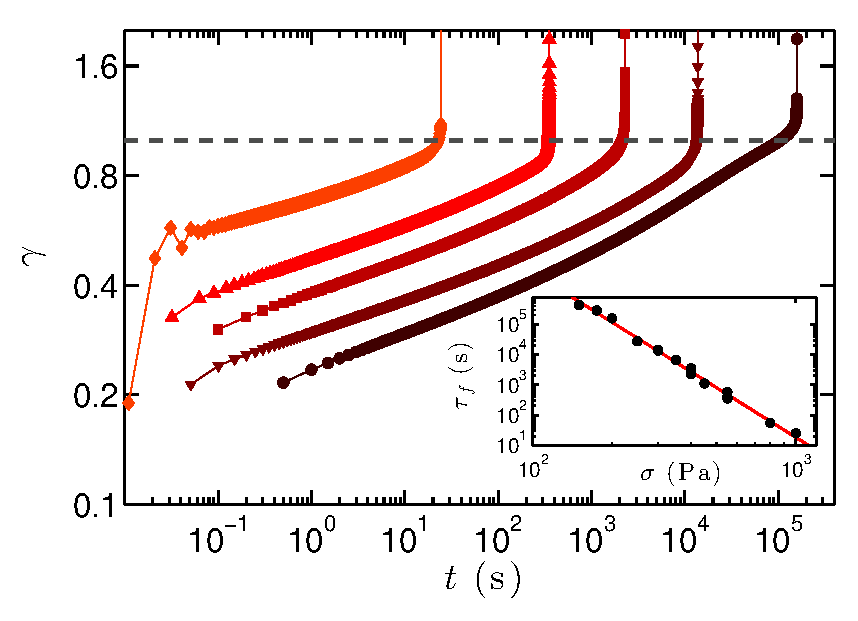
\includegraphics[width=7cm,clip]{Fig1.eps}
\caption{(color online) Strain response $\gamma(t)$ in a 4\%~wt. casein gel acidified with 1\%~wt. GDL for an imposed shear stress $\sigma=200$ ($\bullet$), 300 ($\blacktriangledown$), 400 ($\blacksquare$), 550 ($\blacktriangle$), and 1000~Pa ($\blacklozenge$) from right to left. The gap width is 1~mm. The gray dotted line shows $\gamma=1$. Inset: failure time $\tau_f$ vs $\sigma$. The red line is the best power-law fit $\tau_f=A\sigma^{-\beta}$ with $\beta=5.45\pm 0.05$ and $A=40.6\pm 0.5$~s.Pa$^\beta$.
\label{fig1}}
\end{figure} 
%%%%%%%%%%%%


%%%%%%%%%%%%
\begin{figure}
\centering
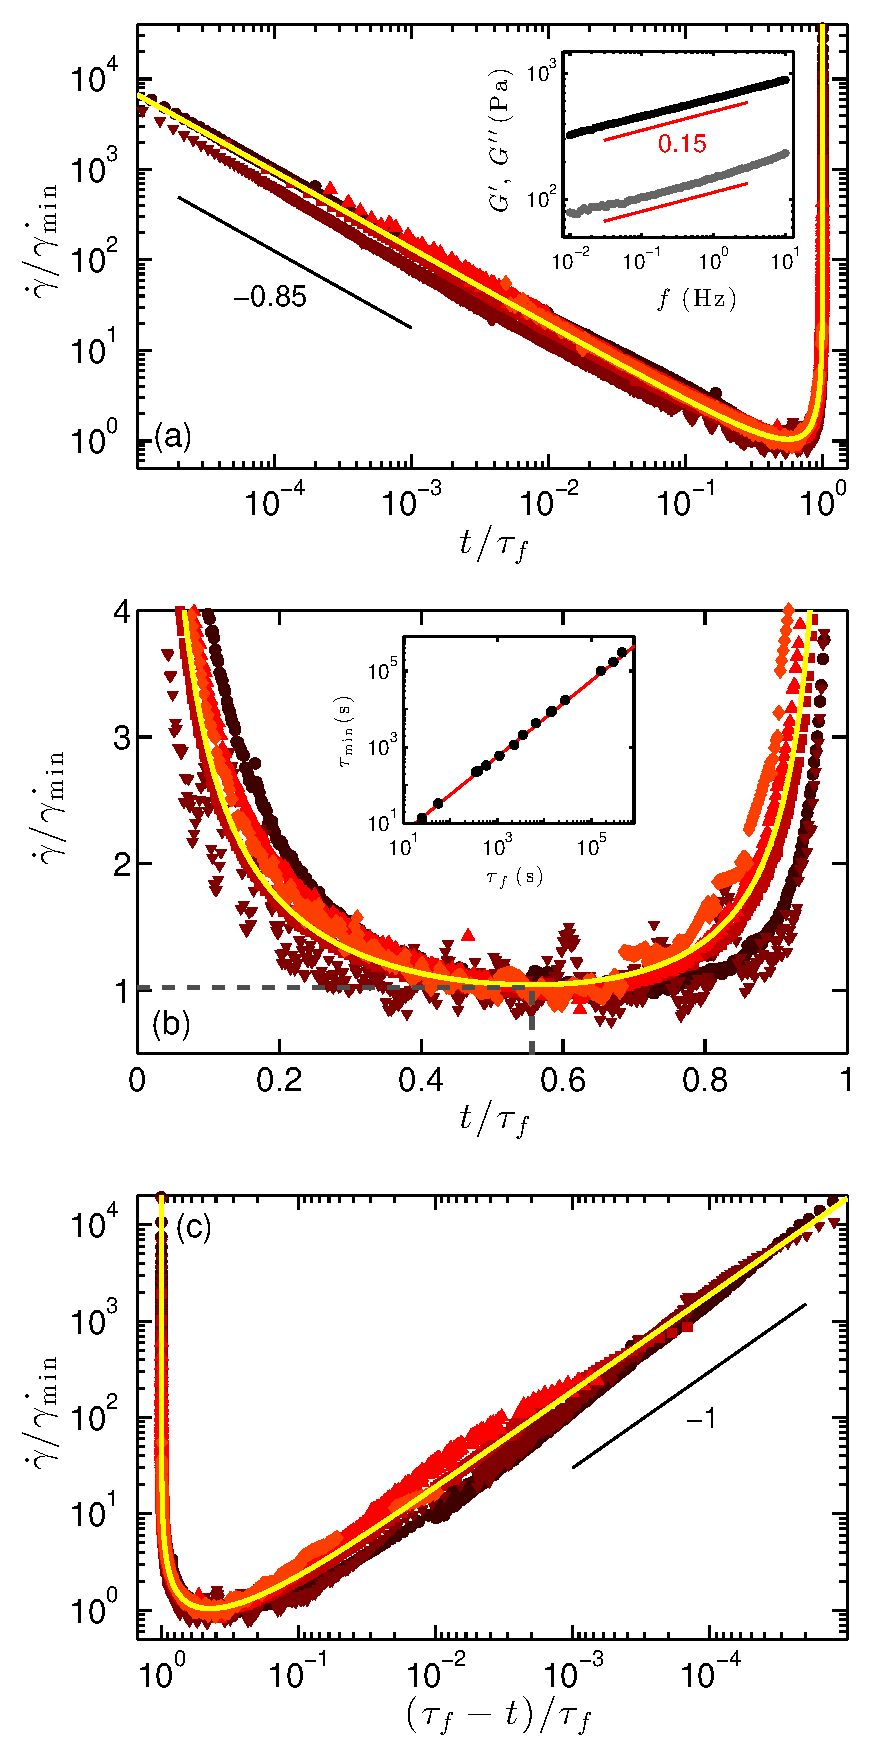
\includegraphics[width=7cm,clip]{Fig2.eps}
\caption{(color online) Normalized shear rate responses $\gp(t)/\gpm$ corresponding to the data of Fig.~\ref{fig1} and plotted so as to emphasize each of the three successive creep regimes. $\gpm$ is the minimum shear rate reached at $\taum$ (see text and Suppl. Fig.~2). (a)~Primary creep: $\gp(t)/\gpm$ vs $t/\tau_f$ in logarithmic scales. The yellow line is $\gp(t)\sim t^{-0.85}$. Inset: Linear viscoelastic moduli $G'$ (top) and $G''$ (bottom) as a function of frequency $f$ for a strain amplitude of 1XXX~\%. Red lines are power laws $G'\sim G''\sim f^{0.15}$. (b)~Secondary creep: $\gp(t)/\gpm$ vs $t/\tau_f$ in linear scales. The yellow curve is a sixth order polynomial fit to the data showing that $\taum\simeq 0.6\tau_f$. Inset: $\taum$ vs $\tau_f$. The red line is the best linear fit $\taum=0.598\tau_f$. (c)~Tertiary creep: $\gp(t)/\gpm$ vs $(\tau_f-t)/\tau_f$ in logarithmic scales with a reversed horizontal axis. The yellow line is $\gp(t)\sim (\tau_f-t)^{-1}$. 
\label{fig2}}
\end{figure} 
%%%%%%%%%%%%

%%%%%%%%%%%%
\begin{figure*}
\centering
\includegraphics[width=18cm,clip]{Fig3.eps}
\caption{(color online) Ultrasonic images (left) and direct visualization of the Couette cell (right) recorded simultaneously at various times in the primary [(a)~$t/\tau_f=0.02$], secondary [(b)~$t/\tau_f=0.57\simeq\taum/\tau_f$], and tertiary  [(c) $t/\tau_f=0.93$ and (d) 0.99] creep regimes. Ultrasonic images are velocity maps $v(r,z,t)$ computed by averaging over 4~s and coded using the linear color levels shown below the images, whose position relative to the picture of the cell reflects the actual arrangement of the ultrasonic probe along the vertical direction $z$. Experiment performed on a 4\%~wt. casein gel seeded with 3\%~wt. polyamide spheres and acidified with 1\%~wt. GDL under $\sigma=300$~Pa. The gap width is 2~mm. See also Suppl. Movie~1.
\label{fig3}}
\end{figure*} 
%%%%%%%%%%%%

%%%%%%%%%%%%
\begin{figure*}
\centering
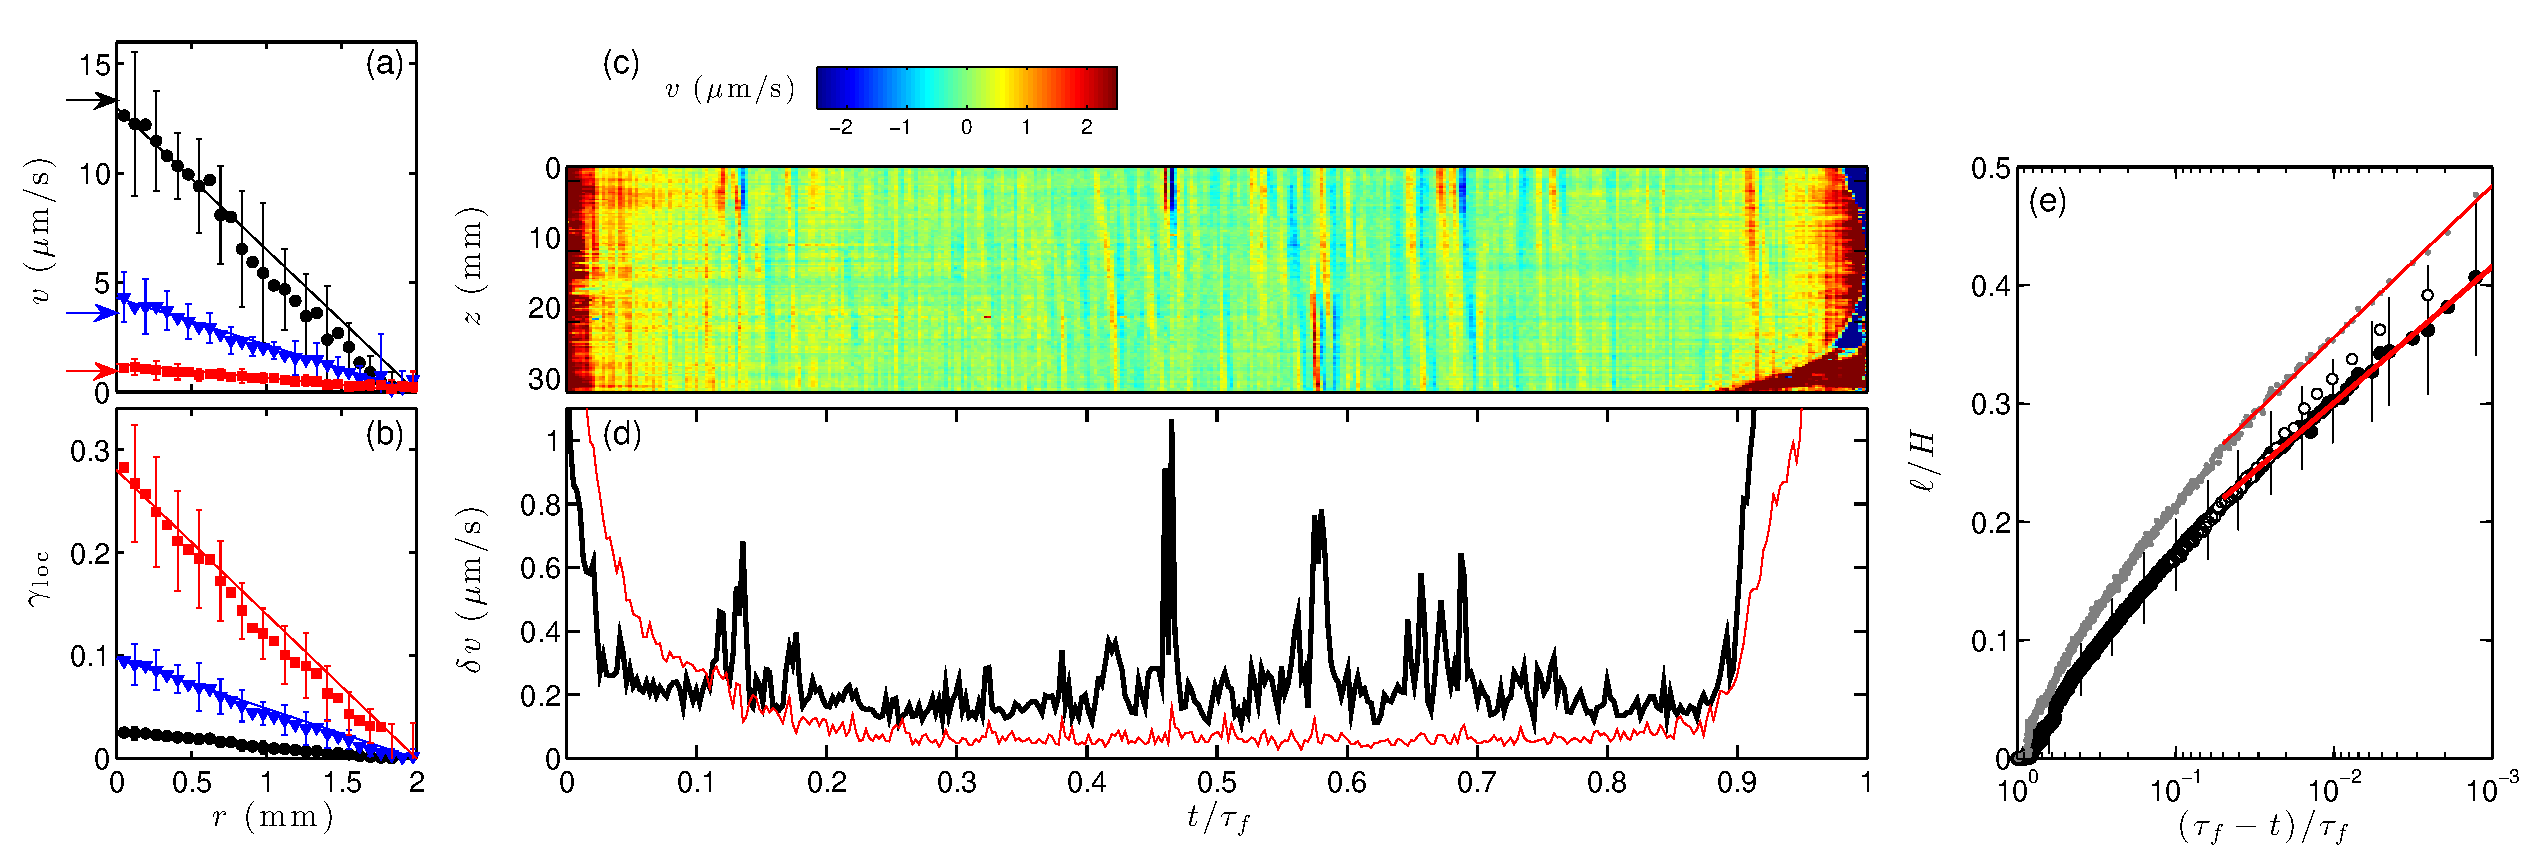
\includegraphics[width=18cm,clip]{Fig4.eps}
\caption{(color online) (a)~Local velocity $\langle v(r,z,t)\rangle_z$ and (b)~local strain field $\langle\gl(r,z,t)\rangle_z$ averaged over the vertical direction $z$ at various times during primary creep: $t/\tau_f=1.9\,10^{-3}$ (black $\bullet$), $1.7\,10^{-2}$ (blue $\blacktriangledown$), and 0.15 (red $\blacksquare$). Solid lines are linear profiles. (c)~Spatiotemporal diagram of the local velocity $\langle v(r,z,t)\rangle_r$ averaged over the radial direction $r$ and plotted in linear color levels as a function of $z$ and $t/\tau_f$. (d)~Standard deviation $\delta_z v(t)$ of $\langle v(r,z,t)\rangle_r$ taken over the vertical direction $z$ (thick black line) together with corresponding standard deviation $\delta_r v(t)$ computed over the radial direction $r$ on the $z$-average $\langle v(r,z,t)\rangle_z$ (thin red line). (e)~Fracture length $\ell(t)$ vs $(\tau_f-t)/\tau_f$ as inferred from direct visualization ($\bullet$, average over 6 different fractures, error bars show the standard deviation) and from ultrasonic imaging ($\circ$) and normalized by the height $H$ of the Couette cell. Gray dots show the visualization data for the longest fracture which leads to the failure of the sample at $\tau_f$. Red lines are the best fits $\ell(t)=\alpha+\beta\log(1-t/\tau_f)$ to the visualization data. Same experiment as in Fig.~\ref{fig3}. See also Suppl. Movie~1.
\label{fig4}}
\end{figure*} 
%%%%%%%%%%%%

\begin{acknowledgments}
The authors thank Thomas Gibaud for fruitful discussions and Alan Parker for precious advice and for providing the casein and GDL. This work was funded by the Institut Universitaire de France and by the European Research Council under the European Union's Seventh Framework Programme (FP7/2007-2013) / ERC grant agreement No.~258803. 
\end{acknowledgments}

\bibliography{../../bibseb} 
%\bibliographystyle{jfm}

\clearpage
\newpage
\setcounter{figure}{0}

\section*{\large Supplemental material}

\subsection*{Supplemental movies}

Supplemental Movie~1 shows the creep experiment analyzed in Figs.~\ref{fig3} and \ref{fig4} and performed under $\sigma=300$~Pa on a 4\%~wt. casein gel seeded with 3\%~wt. polyamide spheres and acidified with 1\%~wt. GDL. The gap width of the Couette cell is 2~mm and its height is 60~mm. Images recorded by a standard webcam are shown on the top left. Velocity maps $v(r,z,t)$ inferred from ultrasonic imaging by averaging over 4~s are shown on the top right using linear color levels. The vertical position $z=0$ on the ultrasonic images corresponds to about 20~mm below the top of the Couette cell. The two bottom graphs show the shear rate response $\gp(t)$ (left) and the strain response $\gamma(t)$.

Supplemental Movie~2 shows the failure of a 4\%~wt. casein gel acidified with 1\%~wt. GDL in a plate-plate geometry for an imposed shear stress $\sigma=XXX$~Pa. The plate diameter is 40XXX~mm and the gap width is 1XXX~mm. In this case fractures grow parallel to the vorticitty direction, i.e. along the radial direction. The shear rate response is fully similar to that in the Couette geometry.

\subsection*{Supplemental figures} 

 %%%%%%%%%%%%
\begin{figure}[h]
\centering
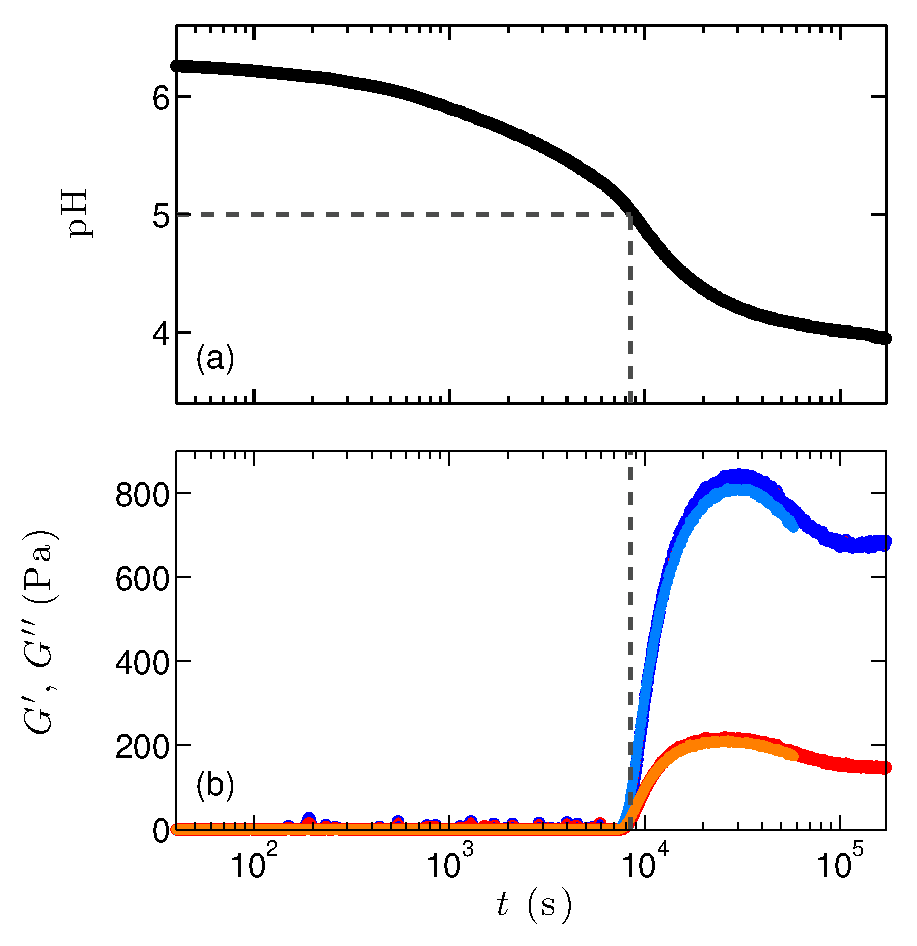
\includegraphics[width=7cm,clip]{SuppFig1.eps}
\caption{(color online) Gelation process of a 4\%~wt. casein suspension seeded with 3\%~wt. polyamide spheres and acidified with 1\%~wt. GDL. (a)~pH vs time $t$. (b)~Linear viscoelastic moduli $G'$ (top, in blue) and $G''$ (bottom, in red) recorded as a function of time $t$ for fixed frequency $f=1$~Hz and strain amplitude 0.1XXX~\%. Dashed lines indicate that the system starts to build significant elastic properties when the pH decreases below about 5. Lighter colors in (b) correspond to a sample free of polyamide spheres, showing that the addition of acoustic contrast agents does not affect significantly the gelation process and the final viscoelastic properties of the gel.
\label{suppfig1}}
\end{figure} 

 %%%%%%%%%%%%
\begin{figure}[h]
\centering
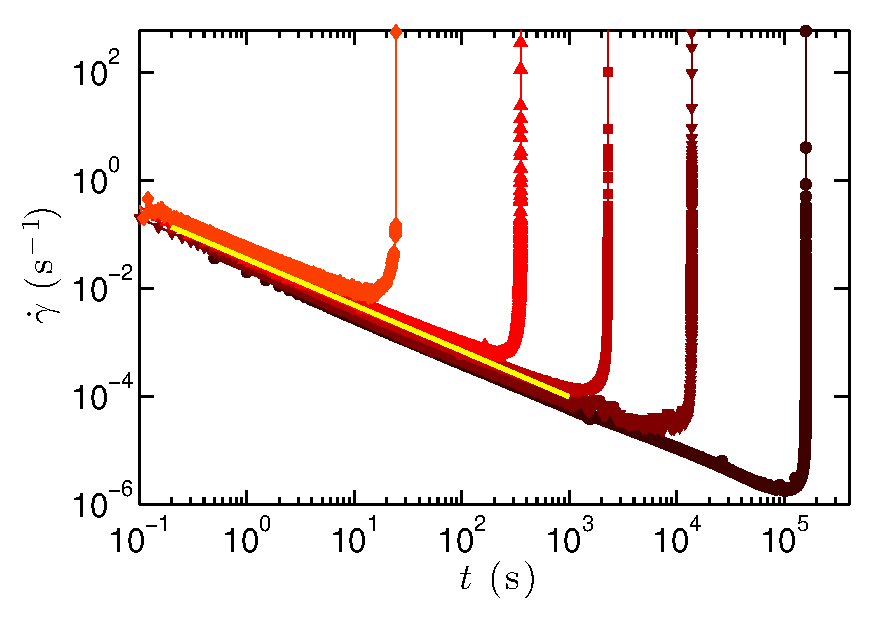
\includegraphics[width=7cm,clip]{SuppFig2.eps}
\caption{(color online) Shear rate response $\gp(t)$ in a 4\%~wt. casein gel acidified with 1\%~wt. GDL for an imposed shear stress $\sigma=200$ ($\bullet$), 300 ($\blacktriangledown$), 400 ($\blacksquare$), 550 ($\blacktriangle$), and 1000~Pa ($\blacklozenge$) from right to left. The gap width is 1~mm. The yellow line shows the power-law behavior $\gp(t)\sim t^{-0.85}$.
\label{suppfig2}}
\end{figure} 
%%%%%%%%%%%%

\end{document}
